\begin{qBox}{4}
Plot the "reduced" correlation function, \( f ( i ) - \langle s \rangle^{ 2 } \),
at \( 0.5 \times T_{ C } \), \( 0.95 \times T_{ C } \), and \( 2 \times T_{ C } \).
Determine the corresponding correlation lengths.

\tcblower

Below are the plot and fitted plot:

\begin{figure}[H]
    \centering
    \begin{minipage}{0.45\linewidth}
        \centering
        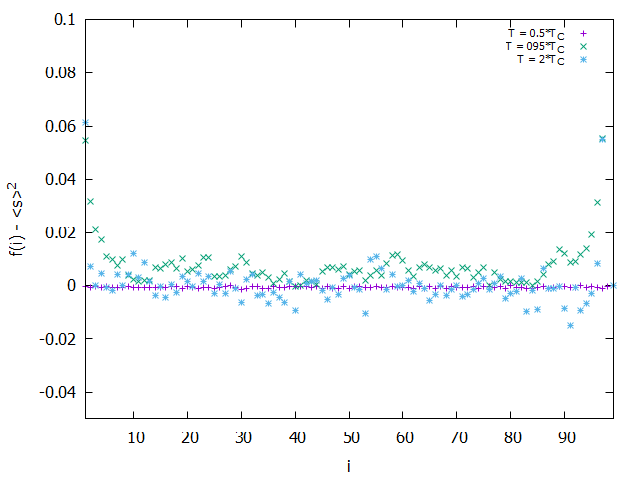
\includegraphics[ width = 0.95\linewidth ]{figures/assignment6_4.png}
        \caption{The plot of the "reduced" correlation function}
    \end{minipage}%
    \begin{minipage}{0.45\linewidth}
        \centering
        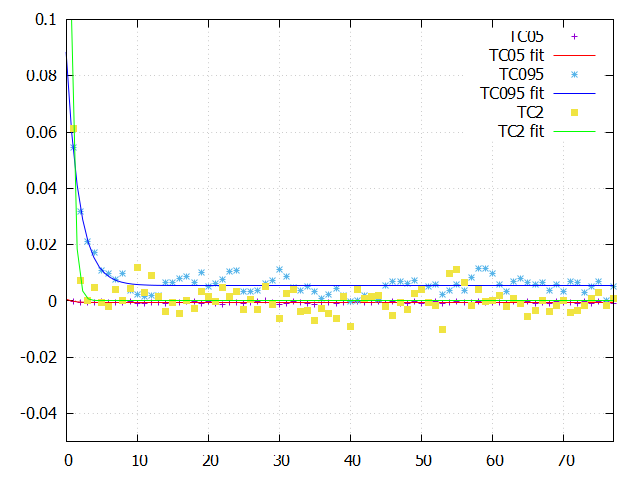
\includegraphics[ width = 0.95\linewidth ]{figures/assignment6_4_fit.png}
        \caption{The fitted plot}
    \end{minipage}%
\end{figure}

As for the fitted values, I got: 
\begin{equation*}
    \begin{aligned}
        0.5 \times T_{ C }&: \xi \approx 0.99533 \pm 7232.49268
        \\
        0.95 \times T_{ C }&: \xi \approx 1.84513 \pm 94.85100
        \\
        2 \times T_{ C }&: \xi \approx 0.46289 \pm 42.46746
    \end{aligned}
\end{equation*}
For the full logs on these fits, they can be found under the log folder.

\baseSkip 

I should note that the fitted values have \textit{very} large uncertainties, so 
we should take these values with a grain of salt (also, the chi-square values for 
these fits were \textit{very} small -- around the order of \( 10^{ -6 } \)).
For how I could have made the fitting better, I think that including weights to these
data point (which is very doable since we are doing many sweeps) would result in a 
fit that has a lower uncertainty; for this fit, I took the weights to be \( 0.5 \) 
for all the points (similar to what was done for the weighted vs. non-weighted 
exponential fits back in lecture 12).
If given more time, I think that I could have implemented this into the fit.

\baseSkip 

However, we see the general relationship between these values to be expected;
as we approach \( T_{ C } \), we should expect \( \xi \) to get larger and larger 
(eventually tending to \( \infty \) as \( T \rightarrow T_{ C } \)).
Indeed, we do see this occurring as \( \xi \) is largest at \( 0.95 \times T_{ C } \)
when compared to the other two correlation lengths. 
Furthermore, we see that the correlation length does seem to be decreasing with 
increasing \( T \), which is what we expected. 

\baseSkip 

As for the correlation length at \( 0.5 \times T_{ C } \) (and its absurdly high 
uncertainty), I think that the value should be more close to \( 0 \) than what is 
found through the fit. 
This is because \( e^{ - r_{ i } / \xi } \approx 0 \) for very small \( \xi \),
which is the trend that we see in the plot. 
Furthermore, we know from lecture that the range and magnitude of the correlation 
length is small at low \( T \), which makes the argument for \( \xi \) being closer to 
\( 0 \) more likely. 

\baseSkip

One final notable trend we see from the plot is that for temperatures near 
\( T_{ C } \), we see that we start with a positive correlation that eventually 
becomes a negative correlation. 
\end{qBox}